\documentclass[]{article}
\usepackage[T1]{fontenc}
\usepackage[utf8]{inputenc}
\usepackage[french]{babel}
\usepackage[]{graphicx}
\usepackage[]{hyperref}

\title{Bilan de projet}
\author{
    Théo Delmas\\
    Lauric Teysseyre\\
    Pierre-Louis Renon\\
    Julien Wattier\\
    \\
    Université Paul Sabatier\\
    Master Informatique 1\\
   } 

\begin{document}
\maketitle
\newpage
\tableofcontents
\newpage

\begin{section}{Objectif du document}
 Ce document présente le bilan du projet.
\end{section}

{
\setlength{\parindent}{0pt} %Retire les alinéas
\begin{section}{Référentiel initial}
 \begin{subsection}{Produits initiaux}
     Le product breakdown initial ainsi que les méthodes de réalisation était les suivants :

     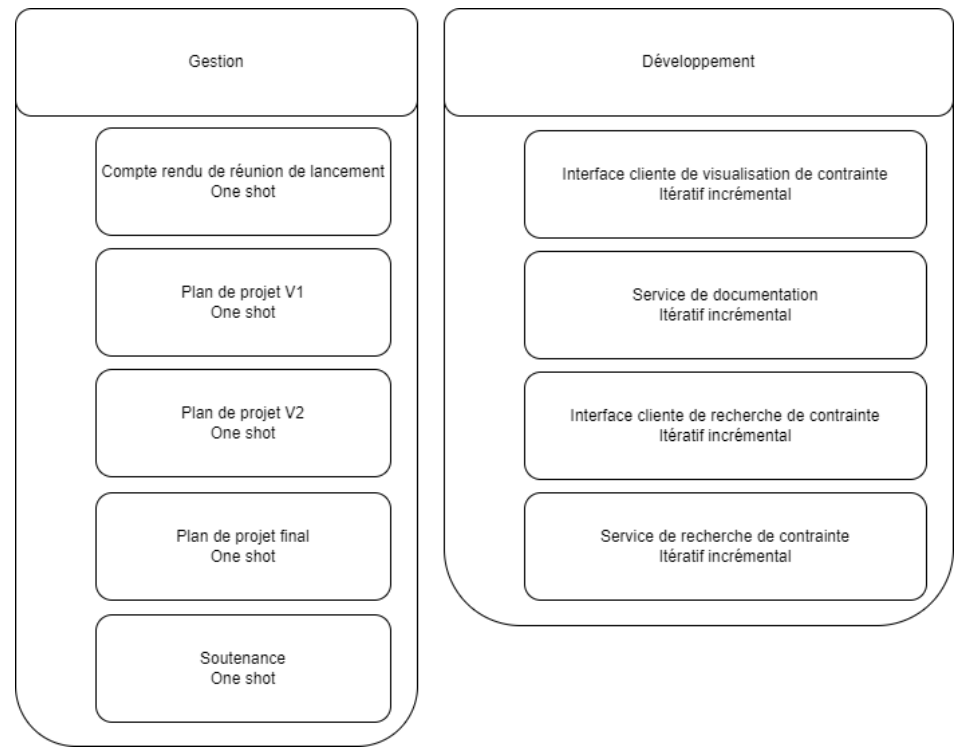
\includegraphics[scale=0.6]{IMG/PBS_initial}
 \end{subsection}
\end{section}

\begin{section}{État courant à la terminaison}
 \begin{subsection}{Produits réalisés}
     L’état des produit à la terminaison du projet sont exposés dans le schéma ci-dessous. Le code couleur indique leur état selon le code suivant :

     \begin{itemize}
         \item Vert : Le produit a été réalisé.
         \item Jaune : Le produit va être réalisé.
         \item Rouge : Le produit n’a pas été réalisé.
     \end{itemize}

     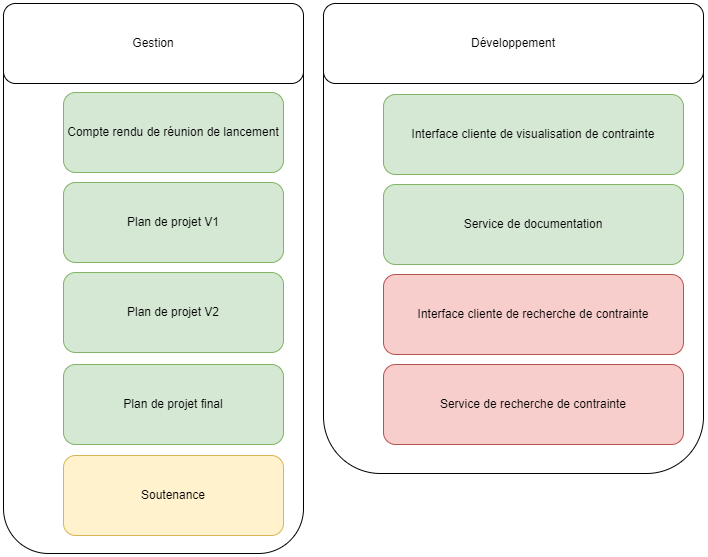
\includegraphics[scale=0.49]{IMG/PBS_final}

     La soutenance va être produit après la clôture du plan projet fixé au 14/03/2023.

     Concernant les produits liés au système de recherche de contrainte, il a été décidé début mars et avec accord du client qu’ils ne seraient pas produits faute de temps.
 \end{subsection}

 \begin{subsection}{Listes des décisions}
     Conformément à la gestion des décision du plan de projet, le \href{Registre_des_décisions.pdf}{registre des décisions} référence l'ensemble des décisions ayant amendé le plan de projet.
 \end{subsection}
\end{section}

\begin{section}{Analyse du déroulement du projet}

\end{section}

\begin{section}{Leçons apprises}

\end{section}

\begin{section}{Perspectives}

\end{section}

\begin{section}{Recommandations}

\end{section}

}
\end{document}